\documentclass[conference]{IEEEtran}
\IEEEoverridecommandlockouts
% The preceding line is only needed to identify funding in the first footnote. If that is unneeded, please comment it out.
\usepackage[acronym]{glossaries}
\usepackage{amsmath,amssymb,amsfonts}
\usepackage{algorithmic}
\usepackage{graphicx}
\usepackage{textcomp}
\usepackage{xcolor}
\usepackage{listings}
\usepackage{biblatex}

\usepackage{todonotes}
\newcommand{\db}[1]{\textcolor{blue!40}{#1}}
\newcommand{\dbc}[1]{\todo[author=Dilum, inline, color=blue!40]{#1}}

\usepackage{hyperref}
\usepackage[noabbrev,capitalise]{cleveref}

\addbibresource{mendeley.bib}

\definecolor{codegreen}{rgb}{0,0.6,0}
\definecolor{backcolour}{rgb}{0.95,0.95,0.92}
\lstdefinestyle{code-style}{
  backgroundcolor=\color{backcolour}, commentstyle=\color{codegreen},
  basicstyle=\ttfamily\footnotesize,
  breakatwhitespace=false,         
  breaklines=true,                 
  captionpos=b,                    
  keepspaces=true,                 
  numbers=left,                    
  numbersep=5pt,
  showspaces=false,
  showstringspaces=false,
  showtabs=false,                  
  tabsize=2
}
\lstset{style=code-style}

\def\BibTeX{{\rm B\kern-.05em{\sc i\kern-.025em b}\kern-.08em
    T\kern-.1667em\lower.7ex\hbox{E}\kern-.125emX}}
\begin{document}

\title{Weather Data Integration and Assimilation System\\
% \thanks{Identify applicable funding agency here. If none, delete this.}
}

\author{\IEEEauthorblockN{Gihan Karunarathne}
\IEEEauthorblockA{\textit{Dept. Computer Science and Engineering} \\
\textit{University of Moratuwa}\\
Katubedda, Sri Lanka \\
gihan.09@cse.mrt.ac.lk}
\and
\IEEEauthorblockN{H.M.N. Dilum Bandara}
\IEEEauthorblockA{\textit{Dept. Computer Science and Engineering} \\
\textit{University of Moratuwa}\\
Katubedda, Sri Lanka \\
dilumb@cse.mrt.ac.lk}
\and
\IEEEauthorblockN{Srikantha Herath}
\IEEEauthorblockA{\textit{Center for Urban Water, Sri Lanka} \\
%\textit{Center for Urban Water, Sri Lanka}\\
Battaramulla, Sri Lanka \\
admin@curwsl.org}
}

\maketitle

%%%%%%%%%%%%%%%%%%%%%%%%%%%%%%%%%%%%%%%%%%%%%%%%%%%%%%%%%%%%%%%%%%%%%%%%%%%%%%%%
\begin{abstract}
%We describe our experience with implementing an extendable open source Weather Data Integration and Assimilation System, which is known as \acrshort{wdias}. It uses the modern architecture pattern such as microservice in order to achieve the scalability, rather using monolithic architecture or client service architecture. It provides a modular approach to integration data from different sources and export into different formats. Also the inbuilt extension module system allow users to add new features. The open source tools that are using for \acrshort{wdias} allows to run on Cloud Computing platforms without much hassle with the auto-scaling feature allow to run \acrshort{wdias} from 1 CPU node to nodes with few hundred CPUs. The paper describes the initial design goals, evolve over few architectures to get desired performance, and explains how the system in way to achieve scalability. Later we analyse the performance test observations with the performance metrics.

\db{Numerical Weather Models (NWMs) utilize data collected via diverse sources such as automated weather stations, radars, air balloons, and satellite images. Prior to using such multimodal data into a NWM, it is necessary to transcode data into a format that can be ingested by the NWM. Moreover, the data integration system’s response time needs to be relatively low to forecast and monitor time-sensitive weather events like hurricanes, storms, and flash floods that require rapid and frequent execution of NWMs. The resulting weather data also need to be accessed by many researchers and third-party applications. Even though there are several weather data integration systems, they are based on monolithic or client-server architectures and are unable to benefit from novel computational models such as cloud computing and containers. Moreover, most of this software is proprietary or closed sourced; hence, it is difficult to customize such software for an island like Sri Lanka with different weather seasons. Therefore, in this research, we propose Weather Data Integration and Assimilation System (WDIAS) that utilizes modern architecture pattern such as microservices to achieve scalability, high availability, and low-cost operation based on cloud computing. WDIAS provides a modular architecture to integrate data from different sources, export into different formats, and the inbuilt extension module system allow users to add new features. We demonstrate the utility of WDIAS using cloud-based experimental setup and weather-related synthetic workloads.}
\end{abstract}

\begin{IEEEkeywords}
\db{Cloud computing, data assimilation, data integration, }
\end{IEEEkeywords}

%%%%%%%%%%%%%%%%%%%%%%%%%%%%%%%%%%%%%%%%%%%%%%%%%%%%%%%%%%%%%%%%%%%%%%%%%%%%%%%%
\section{Introduction}
\label{pse:Introduction}
Weather prediction is essential to reduce impact due to natural disasters and to gain
effectively manage natural resources like water.
Center for Urban Water, Sri Lanka (CUrW-SL) [3] is tasked with the mission to reduce water-related natural disasters in Sri Lanka.
It collected real-time data from weather stations and other government entities and generates daily forecasts. Then the generated results are shared with relevant public departments responsible for disaster planning, mitigation, and management.
To enhance the accuracy of weather predictions, it is necessary to provide reliable and
detailed weather data as inputs to NWMs.
Before feeding such diverse data collected from different sources, it is necessary to a data format that can be ingest by the NWMs.
Further these data need to be process with less time, and need to handle bulk stream weather data.

There are many forecasting systems developed with considering above factors for disaster management. The \acrshort{fews} is developed in the Netherland by Deltares for operational forecasting. It uses a model-centric approach with considering forecasting process as a combination of data modeling steps and data transformation algorithms. So, it is a flexible framework with no inherent hydrological modeling capabilities and system and capable of creating forecasting workflows by integrating new models and algorithms. Also it follows a common data-model and allow models to interact with the system via one of the interfaces provided, and all the timeseries data are stored via this common data model. Even this approach is efficient in data storing and accessing, but it has the inherent issues of performance of accessing data via a single data model in a database. One of interesting concept of \acrshort{fews} is using unique fields to identify timeseries such by their location and data type, as well as an id related to the source of the data. Even it provide an simple but most effective feature by following the concept of the open modeling framework proposed by Open model integration \cite{Kokkonen2003InterfacingXML}, the model adapter is causing tide coupling into the execution process with the \acrshort{fews}. This causing some issue with unit testing models separately and does not easily allow users to run the models in flexible manner such as parallel execution or external process.

\acrfull{lead} is using the fundamental concept of  dynamic workflow orchestration and
data management in a Web services framework \cite{Droegemeier2005Service-OrientedWeather}. To predict and analyze weather models
by researchers, it required many resources. Rather than each researcher is running and
handling their computer resources to do the weather experiments, LEAD is providing pool of resources, then the researchers can use this resource a pool to run their
experiment in shorter amounts of time and higher scale. It is following the \acrfull{soa} with different service layers, and expose services via drag and drop interface to create new flow by users to run new forecast workflows. Workflow service in the \acrshort{lead} schedule and run those with promising the full use of underline resources in the system. \acrfull{dias} and \acrfull{madis} mostly provide the functionality of integration and sharing of data. When compared to other systems, those do not have the workflow capabilities. To store on the large volume of disk space, \acrshort{dias} converts the data via a provided set of \acrshort{api}s and provide the functionality of quality control of the data, and metadata management and  shares the data via the Shared API layer. \acrshort{madis} also store the data by converting the data into a common format, and provide access to the data based on role access.

Even though there are many data integration systems, most of them are proprietary or closed source.
For an island like Sri Lanka that having different kinds of weather seasons
over the year than that software originated need to be highly customized.
Thus it required to get support from the vendor to integrate and configure the
system.
And most of the software existing out there is not up to date with the latest
technology concepts such as Cloud Computing.
The modern architecture pattern such as microservice architecture was able to provide high scalability and availability, rather using monolithic architecture or client service architecture.
Since most of existing systems are dependent underline infrastructure providers, the users do not have much flexibility to decide the best cost-effective way to host it. Above facts has been considered while we proposed the \acrfull{wdias}. The main purpose of this system is to design and implement an extendable weather data integration, assimilation, and dissemination system which is capable of handling bulk data efficiently with providing scalability and high throughput with using open source tools and modern cloud computing technologies.

TODO: Update content as below, overview of rest of the paper
This paper first provides a short review of the operational forecasting process and the role of Delft-FEWS within that process. Section 3 provides an overview of the philosophy and the most important components and features of Delft-FEWS, while Section 4 discusses some example applications of the Delft-FEWS system in research and operations. A discussion of the systems strengths and limitations is provided in Section 5. Section 6 finally provides a summary of the paper, as well as an outlook on the future development of Delft-FEWS.

This paper first provides a brief review on necessity of weather forecasting and some of existing weather data systems. \cref{pse:background} provides an overview of modern architectural patterns used in \acrshort{wdias} and the important components and features of the \acrshort{wdias} discussed in \cref{pse:wdias_architecture}, next \cref{pse:performance_analysis} discusses the test workload performance analysis with comparing with the metrics. 
%%%%%%%%%%%%%%%%%%%%%%%%%%%%%%%%%%%%%%%%%%%%%%%%%%%%%%%%%%%%%%%%%%%%%%%%%%%%%%%%
\section{\db{Background}}
\label{pse:background}

\cref{fi:wdia_components} shows the basic functions of a Weather data integration and assimilation system such as Integration, Assimilation, and Dissemination.

\begin{figure}[htbp]
\centerline{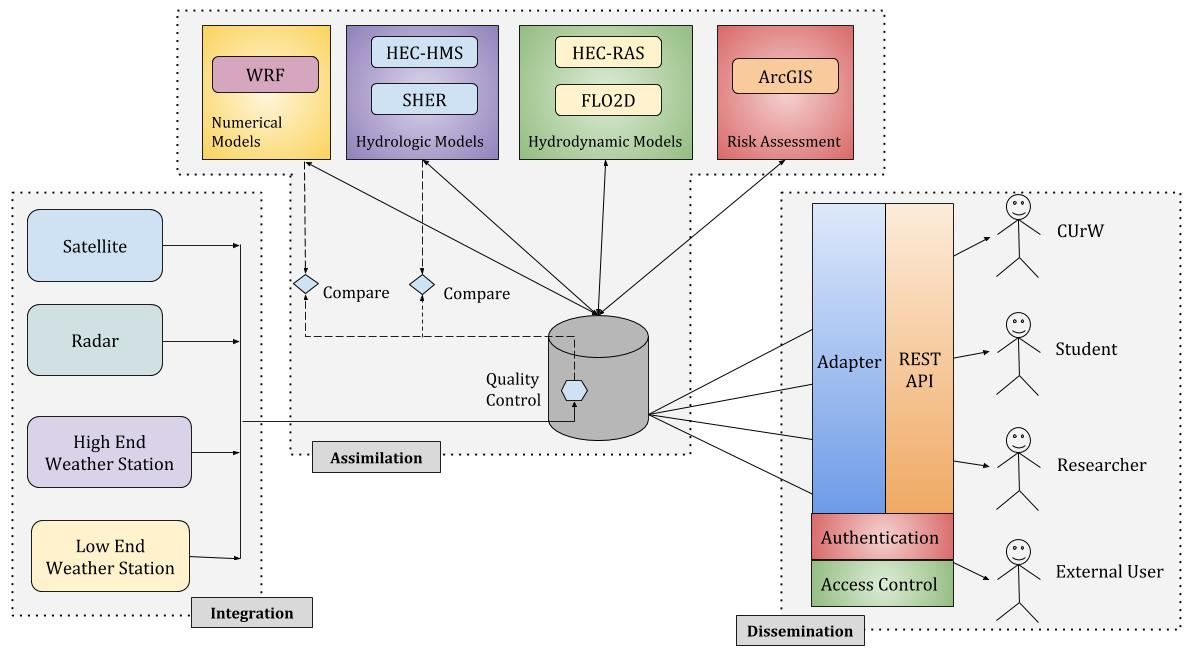
\includegraphics[width=0.5\textwidth]{method/misc/weather_data_system_components.jpg}}
\caption{Components of a weather data system.}
\label{pfi:wdia_components}
\end{figure}

The system should capable of integrating data from different source such as satellite data, high end and low end weather station etc in the form of multidimensional spatial and temporal weather data as shown in the \emph{Integration} modules.
Then the system should be able to fulfill weather models varying data requirements and should be able to store large set of redundant model data during the \emph{Assimilation} module.
The users should be able to easy to search into the available that in the system base on timeseries metadata or based on Geo queries, and the \emph{Dissemination} module should be capable of sharing data among different users.

The \acrshort{wdias} is supporting all three above modules. It iterate through few architectures with concerning about the scalability and high availability.
The initial design of WDIAS used the Service Oriented Architecture (SOA). Moreover, it tried to use an Enterprise Service Bus (ESB) to integrate different modules, as ESB is acting as a common layer for all of the modules. However, it turned out that ESB is not suitable for data streaming or bulk data processing and ESB suffers from a single point of failure since it is using a common bus.
In the second design phase of WDIAS, we attempted to use the actor model using the AKKA framework [9] to overcome above ESB drawbacks and followed the microservice architecture. The system architecture redesign with decomposing into microservices and
used actors to implement each microservice in the system.

Microservice architecture is resilient and flexible as one service is independent of another service. And it is highly scalable as demanding services can be deployed in multiple servers. One of the attractive features of microservice architecture is the independent nature of the microservices which allows to choose different technologies and maintain separately. But using AKKA framework for implement microservice architecture has some disadvantages such as unable to choose independent technologies and the actors messaging between different services cause to result in a too-tight code coupling between the services. To overcome these issues, we moved to the concept of container orchestration based microservice architecture.

%%%%%%%%%%%%%%%%%%%%%%%%%%%%%%%%%%%%%%%%%%%%%%%%%%%%%%%%%%%%%%%%%%%%%%%%%%%%%%%%
\subsection{Microservice Architecture}
\label{psubse:microservice_architecture}

A microservice architecture style is an approach to developing a single application as
a suite of small services, each running in its own process and communicating with
lightweight mechanisms, often via providing a RESTful API. Follow are some of the microservice design patterns mostly used in the context of designing WDIAS architecture.
\begin{itemize}
    \item \emph{Smart Endpoints and Dumb Pipes} - rather than implementing smart endpoints with supporting multiple protocols and complex logic, microservices aim to be as decoupled and as cohesive as possible with only focusing one own domain.
    \item \emph{Database per microservice} - The idea is to keep each microservices persistent data private to that service and accessible only via its API.
    \item \emph{Distributed Transactions over microservices via event processing} - A service publishes an event when its data changes. Other services consume that event and update their data.
    \item \emph{X-axis Scaling} -  running multiple copies of an application behind a load balancer
    \item \emph{Y-axis Scaling} - splits the application into multiple, different services. Each service is responsible for one or more closely related functions. The microservice architecture is an application of Y-axis scaling.
    \item \emph{Z-axis Scaling} - each server runs an identical copy of the code (similar to X-axis scaling). The big difference is that each server is responsible for only a subset of the data.
\end{itemize}

The \acrshort{wdias} is using \acrfull{k8s} as the container orchestration system which is an open-source tool for automating deployment, scaling, and management of containerized applications.

\begin{figure}[htbp]
\centerline{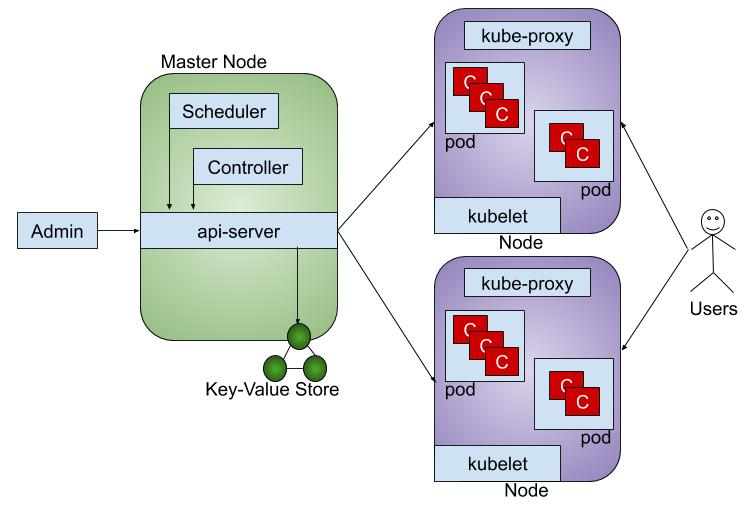
\includegraphics[width=0.5\textwidth]{method/microservice/k8s_architecture_v3.jpg}}
\caption{\acrfull{k8s} architecture.}
\label{pfi:k8s_architecture}
\end{figure}

\cref{fi:k8s_architecture} gives an overall idea on the components of \acrshort{k8s},
\begin{itemize}
    \item Pods -- Cluster of containers that can group other container images in a single unit.
    \item Nodes -- the machines (VMs, physical servers, etc) in a cluster that runs your applications and cloud workflows.
    \item kubelet -- An agent that runs on each node in the cluster. It makes sure that containers are running in a pod.
    \item kube-proxy -- A network proxy that runs on each node in the cluster, and maintains network rules on nodes.
    \item Kubernetes master -- Responsible for maintaining the desired state for your cluster.
    \item etcd -- Consistent and highly-available key value store used as Kubernetes’ backing store for all cluster data.
\end{itemize}
Users can add much as required Nodes into the K8s cluster, and K8s manage and
deploy applications as pods into cluster nodes. Thus it allow users to implement the microservice architecture concepts above easily.

%%%%%%%%%%%%%%%%%%%%%%%%%%%%%%%%%%%%%%%%%%%%%%%%%%%%%%%%%%%%%%%%%%%%%%%%%%%%%%%%
\section{\acrfull{wdias} Architecture}
\label{pse:wdias_architecture}



\begin{figure}[htbp]
\centerline{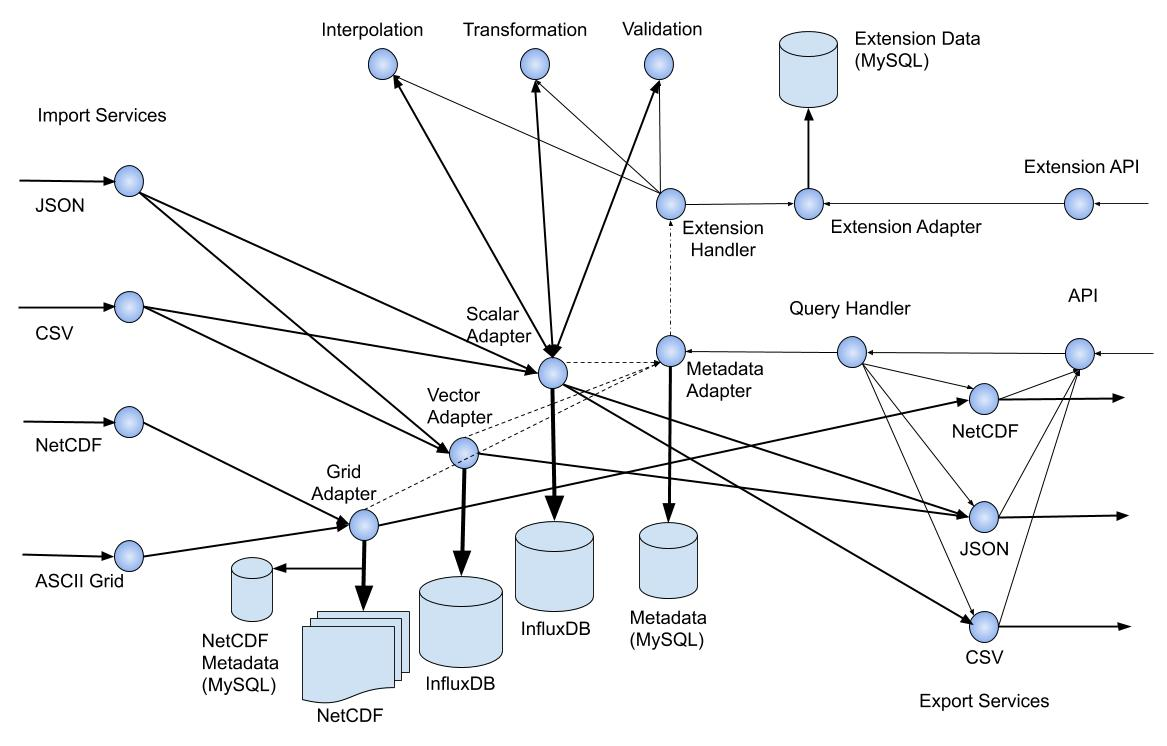
\includegraphics[width=0.5\textwidth]{method/microservice/microservice_architecture-handle_on_demand-v3.jpg}}
\caption{microservice architecture - handle on demand.}
\label{pfi:microservice_architecture_on_demand}
\end{figure}

\begin{figure}[htbp]
\centerline{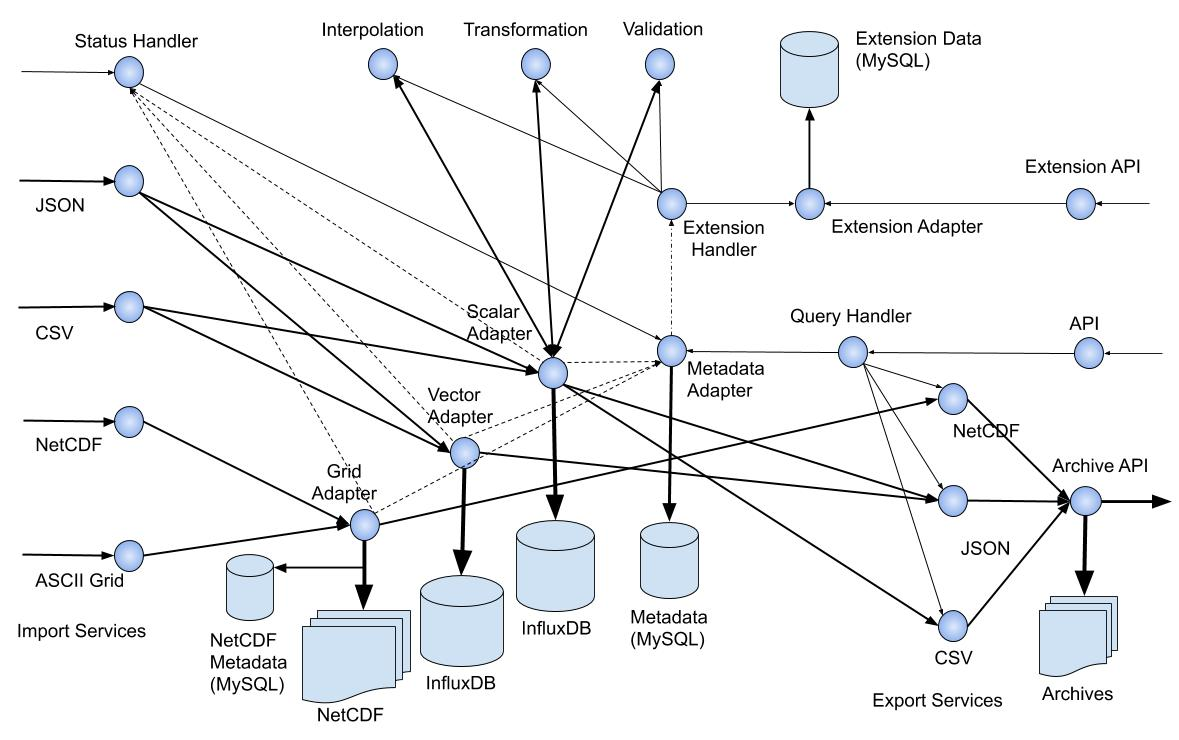
\includegraphics[width=0.5\textwidth]{method/microservice/microservice_architecture-handle_on_async-v3.jpg}}
\caption{microservice architecture - handle asynchronously.}
\label{pfi:microservice_architecture_async}
\end{figure}

%%%%%%%%%%%%%%%%%%%%%%%%%%%%%%%%%%%%%%%%%%%%%%%%
\subsection{\acrshort{wdias} Database Structure}
\label{subse:wdias_database}
\begin{figure}[htbp]
\centerline{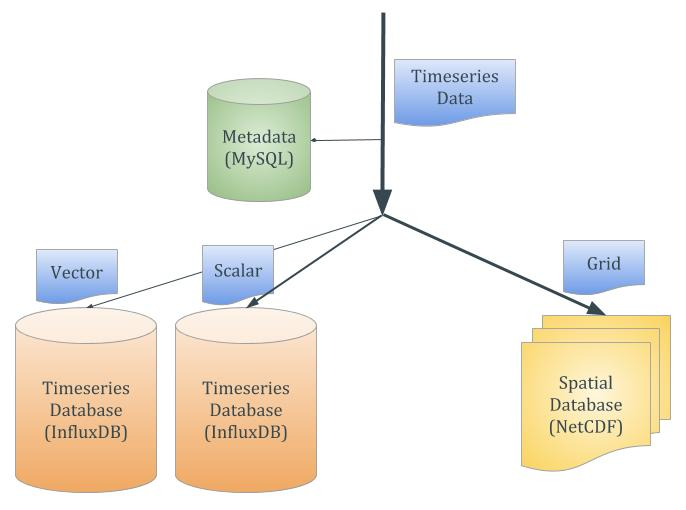
\includegraphics[width=0.4\textwidth]{method/microservice/wdias_database_structure.jpg}}
\caption{Hierarchical database.}
\label{pfi:hierarchical_database}
\end{figure}

%%%%%%%%%%%%%%%%%%%%%%%%%%%%%%%%%%%%%%%%%%%%%%%%
\subsection{Weather Data Preprocessing}
\label{psubse:data_preprocessing}

\begin{figure}[htbp]
\centerline{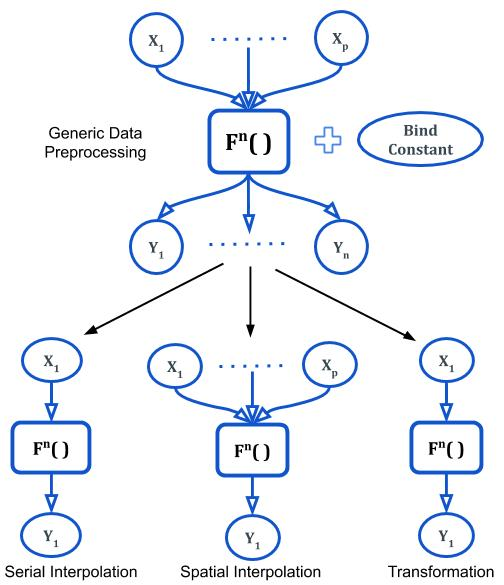
\includegraphics[width=0.4\textwidth]{method/data_preprocess/summary_weather_data_preprocessing.jpg}}
\caption{Generic functional approach to weather data preprocessing.}
\label{pfi:summary_weather_data_preprocessing}
\end{figure}

%%%%%%%%%%%%%%%%%%%%%%%%%%%%%%%%%%%%%%%%%%%%%%%%
\subsection{Query Timeseries Metadata}
\label{psubse:query_timeseries}


%%%%%%%%%%%%%%%%%%%%%%%%%%%%%%%%%%%%%%%%%%%%%%%%%%%%%%%%%%%%%%%%%%%%%%%%%%%%%%%%
\section{Performance Analysis}
\label{pse:performance_analysis}
%\section{Performance Analysis}

%%%%%%%%%%%%%%%%%%%%%%%%%%%%%%%%%%%%%%%%%%%%%%%%
\subsection{Test Plan and Workload}
\begin{figure}[htbp]
\centerline{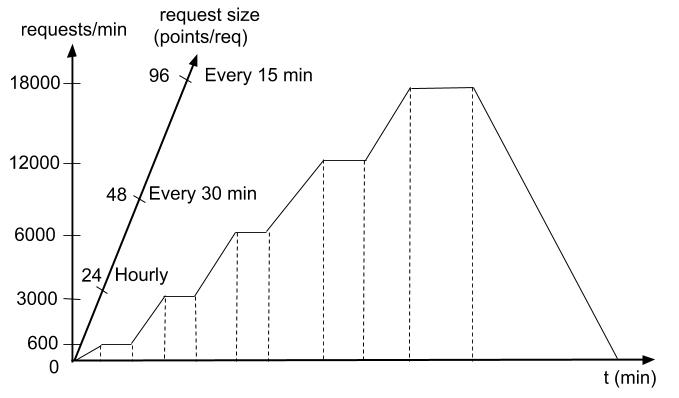
\includegraphics[width=0.5\textwidth]{results/work_load/performance_study_v4.jpg}}
\caption{Performance study.}
\label{pfi:performance_Study}
\end{figure}

%%%%%%%%%%%%%%%%%%%%%%%%%%%%%%%%%%%%%%%%%%%%%%%%
\subsection{Performance Evaluation}
\label{psubse:performance_evaluation}
\begin{table}[htbp]
\caption{Table type styles}
\begin{center}
\begin{tabular}{|c|c|c|c|c|c|c|}
\hline
\textbf{Label} & \textbf{Samples} & \textbf{Avg} & \textbf{Min} & \textbf{Max} & \textbf{Std} & \textbf{90\% Line} \\ \hline
Insert Scalar & 71727 & 34 & 13 & 1777 & 118.78 & 27 \\ \hline
Retrieve Scalar & 71693 & 7 & 5 & 1608 & 18.72 & 9 \\ \hline
Insert Grid & 7968 & 87 & 77 & 233 & 14.07 & 98 \\ \hline
Retrieve Grid & 7965 & 89 & 63 & 1694 & 37.79 & 110 \\ \hline
Query & 71704 & 1 & 0 & 203 & 2.05 & 2 \\ \hline
\textbf{TOTAL} & 310734 & 130 & 0 & 1777 & 212.35 & 501 \\ \hline
\multicolumn{4}{l}{$^{\mathrm{a}}$Avg: Average Latency, Std: Standard Deviation.}
\end{tabular}
\label{ptab:obs_all_auto_15_min_summary_latency}
\end{center}
\end{table}

\begin{table}[htbp]
\caption{Table type styles}
\begin{center}
\begin{tabular}{|c|c|c|c|c|c|}
\hline
\textbf{Label} & \textbf{Samples} & \textbf{Avg} & \textbf{Std. Dev.} & \textbf{Error \%} & \textbf{RPS} \\ \hline
Insert Scalar & 71727 & 34 & 118.78 & 0.00\% & 40.5 \\ \hline
Retrieve Vector & 71693 & 7 & 18.72 & 0.00\% & 40.5 \\ \hline
Insert Grid & 7968 & 87 & 14.07 & 0.18\% & 4.5 \\ \hline
Retrieve Grid & 7965 & 89 & 37.79 & 0.00\% & 4.5 \\ \hline
Query & 71704 & 1 & 2.05 & 0.00\% & 40.5 \\ \hline
\textbf{TOTAL} & 310734 & 130 & 212.35 & 0.00\% & 175.3 \\ \hline
\multicolumn{4}{l}{$^{\mathrm{a}}$Avg: Average Latency.}
\end{tabular}
\label{ptab:obs_all_auto_15_min_summary_throughput}
\end{center}
\end{table}

\begin{figure}[htbp]
\centerline{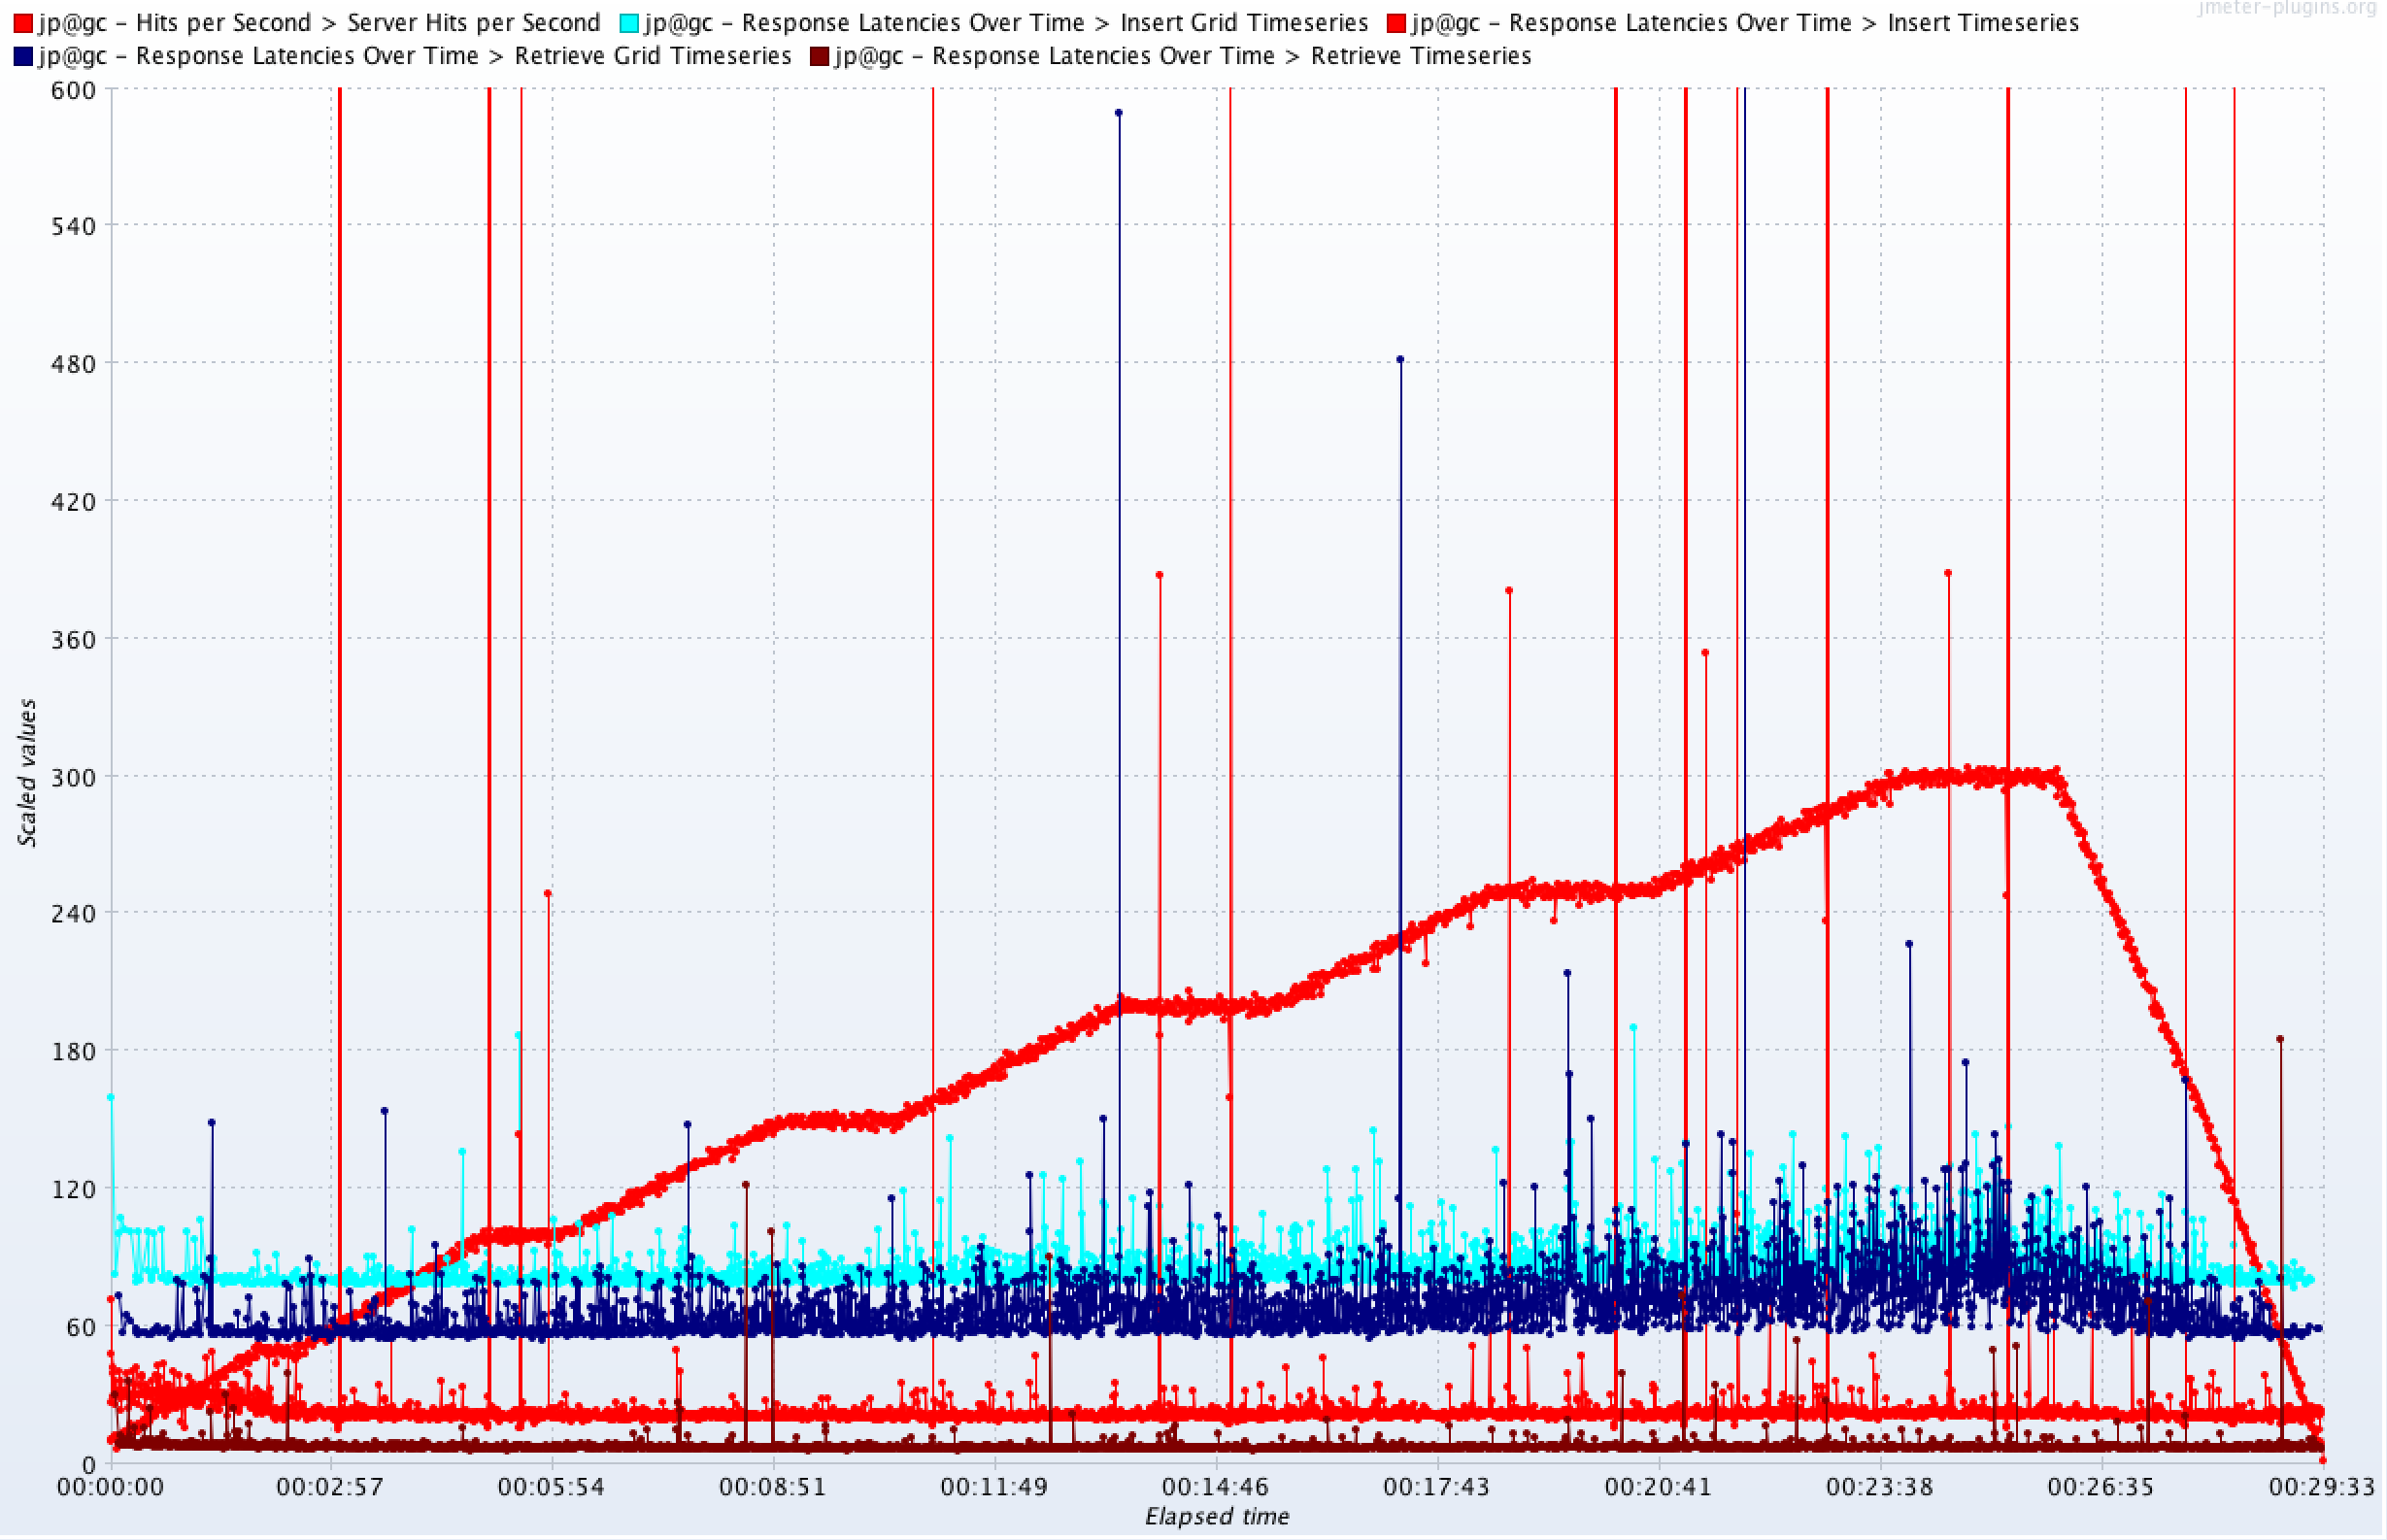
\includegraphics[width=0.5\textwidth]{results/obs/all_auto/obs_all_auto_15m_res_latencies_against_hits.png}}
\caption{Performance test 15min data enabled auto-scaling - response latencies against server hits over the elapsed time.}
\label{pfi:test_obs_auto_all_15_min_latency_vs_hits}
\end{figure}

\begin{figure}[htbp]
\centerline{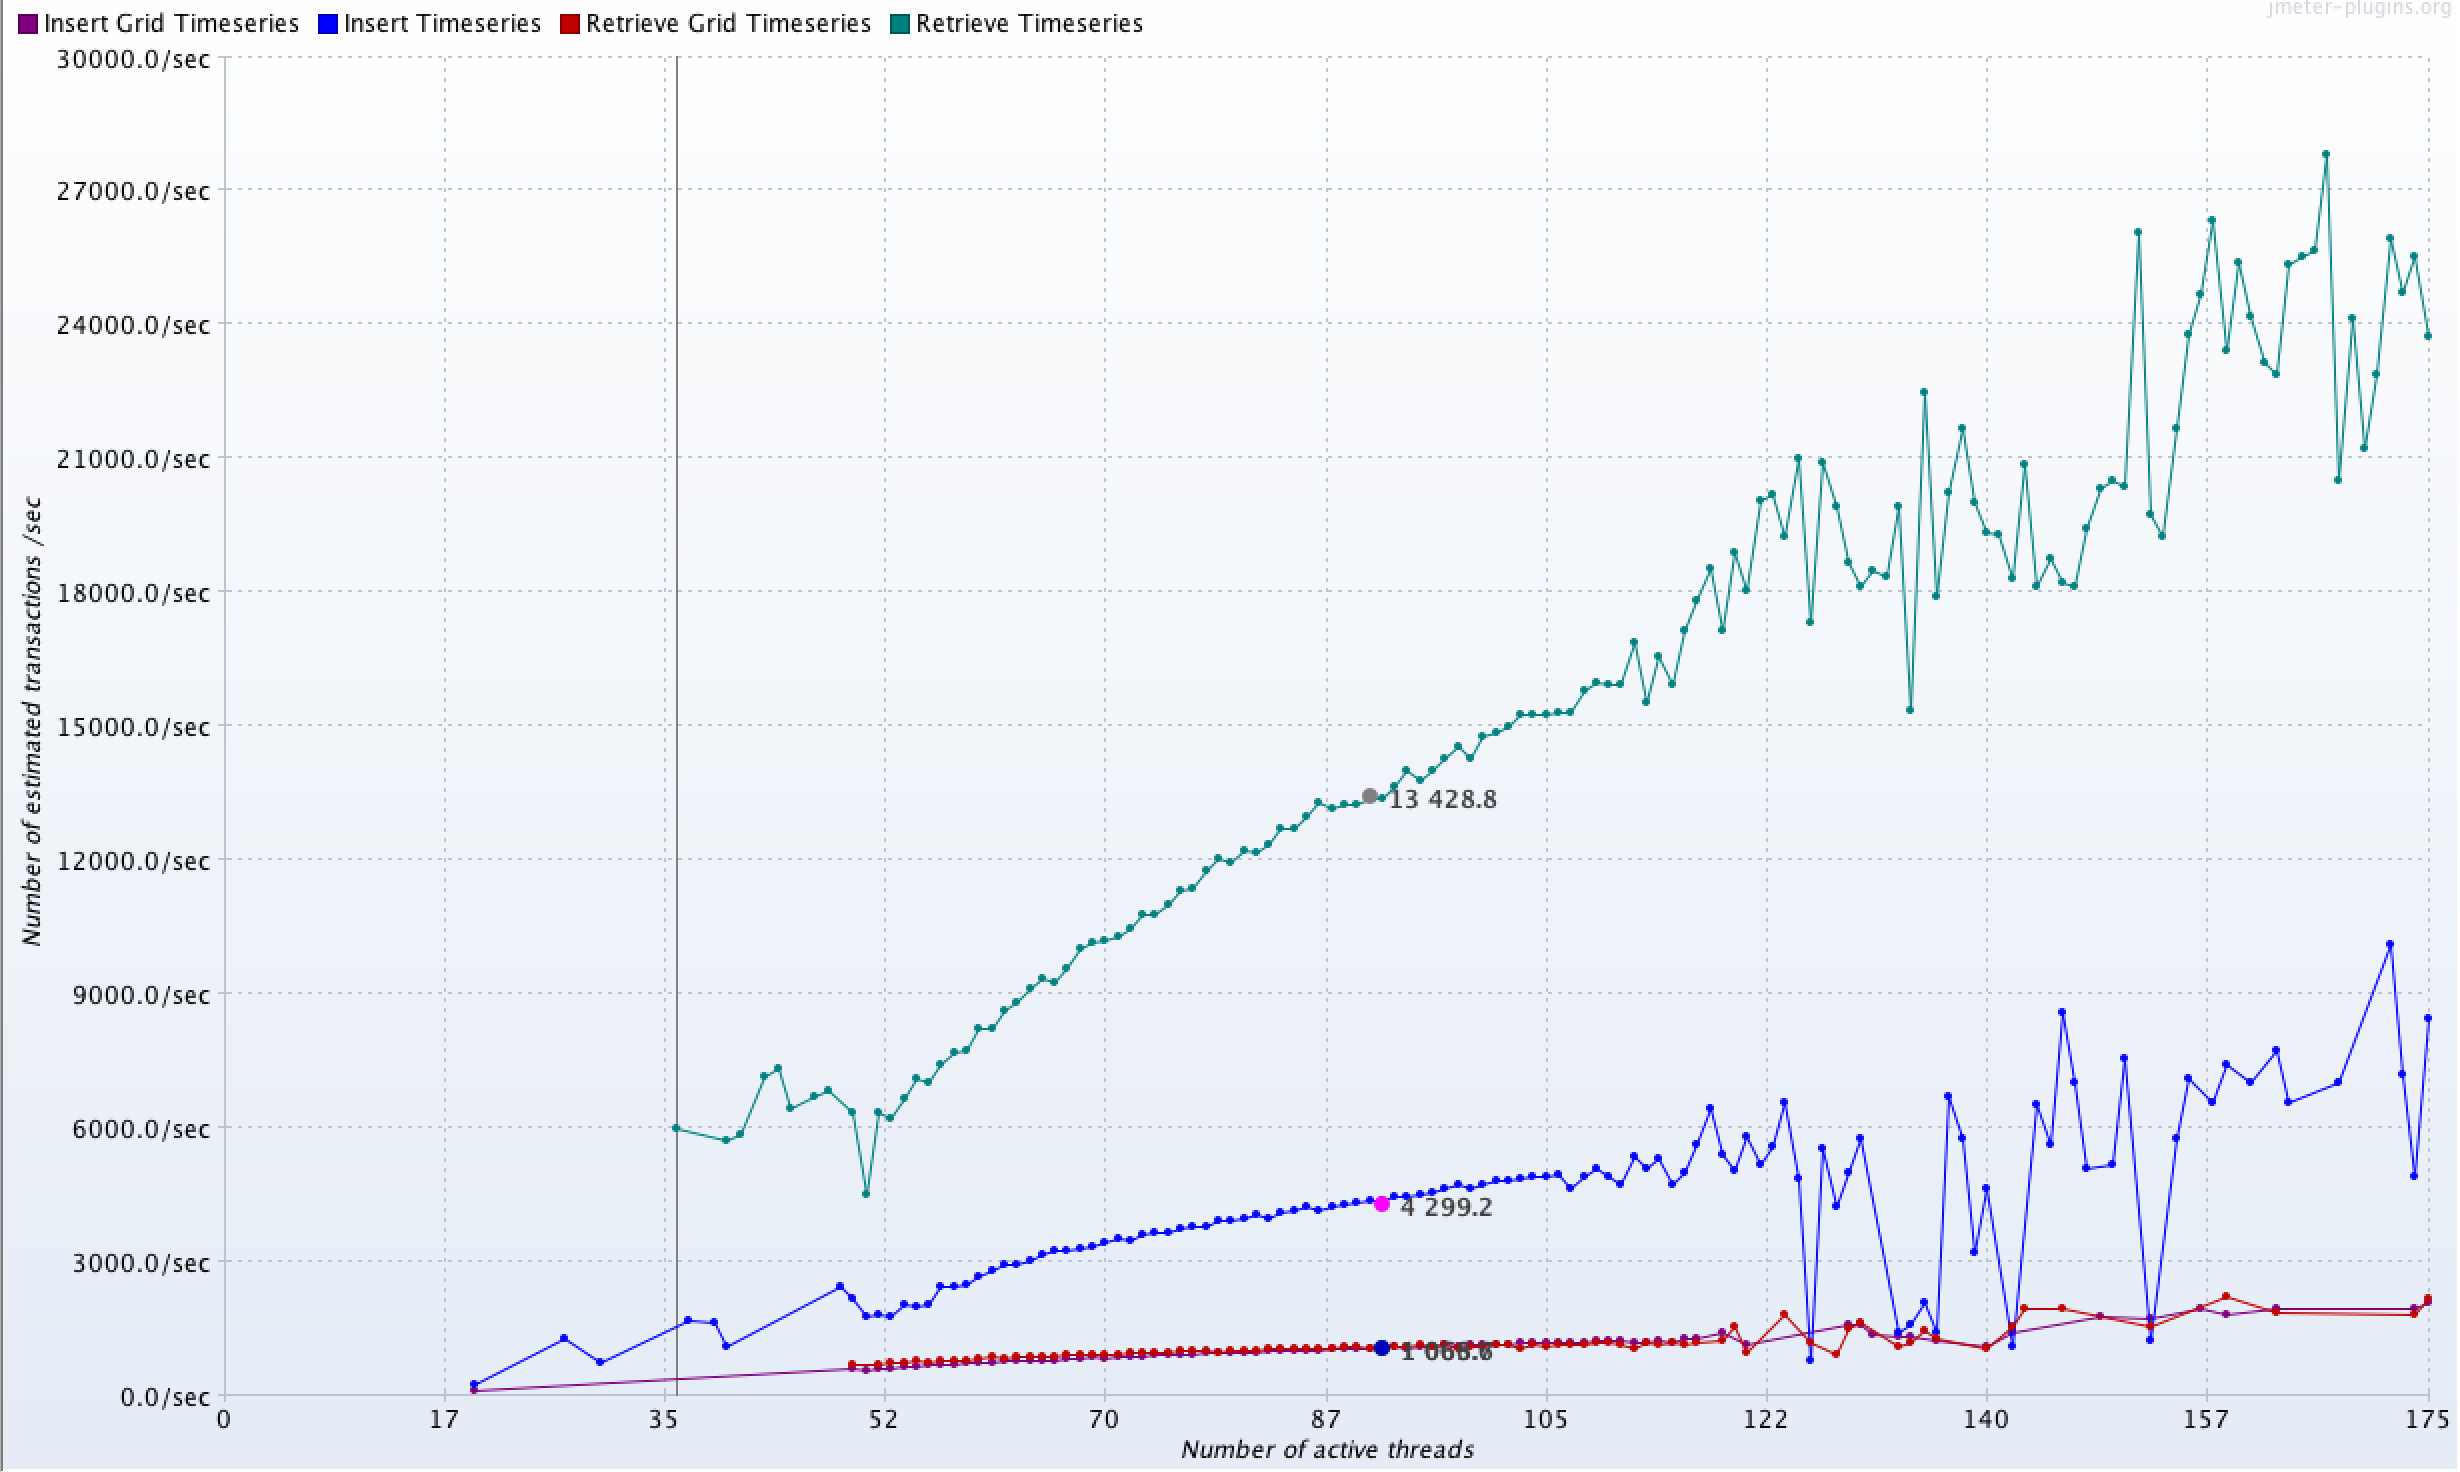
\includegraphics[width=0.5\textwidth]{results/obs/all_auto/obs_all_auto_15m_transaction_throughtput_vs_threads.png}}
\caption{Performance test 15min data enabled auto-scaling - transnational throughput vs number of active threads.}
\label{pfi:test_obs_auto_all_15_min_throughput_vs_threads}
\end{figure}

%%%%%%%%%%%%%%%%%%%%%%%%%%%%%%%%%%%%%%%%%%%%%%%%
\subsection{Performance Metrics Analysis}
\label{psubse:performance_metrics}
\paragraph{Latency}
The latency for each operation type kept constant over the whole test plan run time without any significant change. When the request size increased from 24 data points to 96 data points, the latency increase throughout the whole test plan with a smaller number. But for each test run the latency kept constant over the time.
During the \cref{subse:obs_test_plan_all_auto_15min} test run, the performance of the Grid data got better when compared to the \cref{subse:obs_test_plan_all_15min}. Which means by adding more resources to the \acrshort{wdias}, it can handle more workload on the system.

\paragraph{Throughput}
While keeping the latency constant without significant change, the throughput of the \acrshort{wdias} kept constant while increasing the request size from 60min data (24 data points) to 15min data (96 data points) for all the data types such as Scalar, Vector and Grid.
When number of active threads increased, the \acrshort{wdias} able to provide the same throughput with maintaining the latency stable.

One of the reason to having deviations at the peak time due to use of single instance for the data consistency such as \acrshort{influxdb} for Scalar and Vector data, and netCDF with parallel support for Grid data. Further it is possible to increase the performance of these bottlenecks much higher such as using \acrshort{influxdb} Commercial cluster support for high availability or horizontal scaling of \acrshort{influxdb}. With \acrshort{influxdb} cluster, it is possible to run multiple pods of adapter-scalar and adapter-vector for support more server hits per second.

Adapter-grid is using a Python wrapper for netCDF FORTRAN implementation with parallel IO enabled. This has some performance issues as well as memory leak issues. Since each microservice in the \acrshort{wdias} independent of technology that can use to implement the service, it will increase the performance if the adapter-grid directly ported to netCDF with a low level language such as C or FORTRAN.
Other than \acrshort{eks}, if users can use a \acrshort{k8s} cluster which support Persistent Volumes with the access of Read Write  Many \cite{LinuxFoundationPersistentKubernetes} , then it is possible to run multiple pods of adapter-grid and increase the throughput of the \acrshort{wdias}.

\paragraph{Resource Utilization}
Since \acrshort{wdias} using the \acrshort{k8s} as the container orchestration system, it allows to scale up and cool down the system as required based on the workload. This demonstrate on the test plan of \cref{subse:obs_test_plan_all_auto_15min}, and the system get scale up to the maximum at the peak time. Then cool down to single pod after finishing the test cases.
Given above \acrshort{wdias} can run from 1 CPU node to nodes with 100 CPUs. As described in the \cref{se:microservice}, it uses the many of the concept of modern microservice architecture to create stateless, failover, redundant microservice to achieve such capabilities.

\paragraph{Auto Scaling}
The \acrshort{wdias} supports auto-scaling by out of the box with \acrshort{k8s}. Services can configure with maximum number of pods in order to avoid over resource usage. When there is not much workload on the system, system cool down to less pods in order to save more resources. When there is any issue with a pod, \acrshort{k8s} auto schedule another pod and remove the unhealthy pod. Also it allows to update the system without any down time with rollback updates.

\paragraph{Risk of Unable to Process Data}
During the test performance, the \acrshort{wdias} processed many requests with higher request size than the normal usage with lower rate of failures to process the requests, mainly with insert Grid data. If the usage of \acrshort{wdias} want to reduce the risk of unable to process data, then system can configure to run with redundant pods in order to handle spike of workloads. Also while configure for the auto-scaling, the \acrshort{k8s} can configure to maintain lower amount of CPU usage such as 50\% to 60\% rather 80\%. Such configuration with always spawn new pods to handle double of current peak load.

%%%%%%%%%%%%%%%%%%%%%%%%%%%%%%%%%%%%%%%%%%%%%%%%%%%%%%%%%%%%%%%%%%%%%%%%%%%%%%%%
\subsection{Strengths and Limitations}
\label{psubse:limitations}
\dbc{Make this the dicussion and a sub-section of Sec. 4}

\paragraph{Lack of data preprossessing modules}
The extension module enable plugin system to integrate prepossessing modules which can use for process the data which are inserted to the system or based on regular intervals. Also \acrshort{wdias} provide a more generic open interface approach to create more preprocessing modules. Since \acrshort{wdias} is an open source system, it expect more modules to be create by the community. When compared to other system like \acrshort{fews}, current system only have few extension for the testing purpose. This is one of the major area that need to be improved.

\paragraph{Supporting Irregular Grids}
At the moment \acrshort{wdias} does not support Irregular Grids, but it has the API endpoints define for the implementation which can follow the same microservice architecture. The scope of the \acrshort{wdias} does not belong such level of implementation and the scope has reduced by removing such components from the system.

\paragraph{Grid data performance}
As mentioned in the \cref{se:conclusion}, the adapter-grid is using a Python wrapper for netCDF FORTRAN implementation with parallel IO enabled. This has some performance issues as well as memory leak issues. Since each microservice in the \acrshort{wdias} independent of technology that can use to implement the service, it will increase the performance if the adapter-grid directly ported to netCDF with a low level language such as C or FORTRAN. They are some future work that can focus on improving the performance of grid data.

\paragraph{Define infrastructure as code}
Physical nodes for the \acrshort{k8s} cluster created using Cloud Computing provider such as \acrshort{eks}. And defining the each pod resource limitations at the helm chart level. But the infrastructure that need to deploy the \acrshort{wdias} can define as code such as using tools like Teraform which is independent of the Cloud Computing provider. Using such tool, users will able to easy deploy the \acrshort{wdias} on any Cloud provider without much hassle.

\paragraph{Further improve hierarchical database performance}
As further described in \cref{se:conclusion}, it is possible to increase the performance of these bottlenecks much higher such as using \acrshort{influxdb} Commercial cluster support for high availability or horizontal scaling of \acrshort{influxdb}. With \acrshort{influxdb} cluster, it is possible to run multiple pods of adapter-scalar and adapter-vector for support more server hits per second.
Other than that, the \acrshort{wdias} performance can improve via partitioning the timeseries key space into multiple \acrshort{influxdb} instances. The adapter-scalar or adapter-vector can improve to plug multiple instance of \acrshort{influxdb} instances by changing the configurations. As an example, based on the key attribute \cref{subse:timeseries_key_attributes} Timeseries Type, the adapter-scalar can connect to four instance of \acrshort{influxdb} instances such as  External Historical, External Forecast, Simulated Historical, and Simulated Forecast etc.

%%%%%%%%%%%%%%%%%%%%%%%%%%%%%%%%%%%%%%%%%%%%%%%%%%%%%%%%%%%%%%%%%%%%%%%%%%%%%%%%
\section{Summary}
\label{pse:summary}
\dbc{Summary is too long. Should not be more than a single para}
To enhance the accuracy of the weather prediction, it is required to have reliable weather data for \acrshort{nwm}. Most of existing weather data systems are proprietary or close sourced, or not up to date with the existing cloud computing technologies.
We proposed an extendable open source Weather Data Integration and Assimilation Systems which is known as \acrshort{wdias}. It focused on providing efficiently integrates weather data from different sources with quality control and supporting steaming large size of data. And compatible with current cloud computing technologies and architecture patterns.

First the architecture starts with SOA using a \acrfull{esb}, and then moved to Actor model based architecture. After comparing the disadvantages of using such architecture with the system requirements, final architecture come up with modern microservice architecture.
Based on the microservice architecture patterns and the nature of the weather metadata, the \acrshort{wdias} came up with the idea of hierarchical database structure in order to provide higher performance while store the weather data. The system uses \acrshort{influxdb} timeseries database for storing Scalar and Vector timeseries data, and using \acrshort{netCDF} for storing Grid timeseries data.
Also the system provide a generic open mechanism to integrate new modules as extension in order to enhance the features of the system. This capability enable to integrate weather data preprocessing flows as extension modules.
The extension API provide easy access to create and modify the extension triggers on the fly without stopping the system or any downtime in order to change the configurations.
The system provides extensive timeseries query endpoints to easy search over the system timeseries metadata with supporting Geo based queries.

\acrshort{wdias} performance test is perform using the \acrshort{jmeter} tool's distributed testing capabilities which separately testing each modules. Then the test plans are performed with increasing the request size, and monitored the performance metrics. The system is setup on the \acrfull{eks} as per the configurations of \cref{subse:test_sys_config}.
During the performance test plans, the system were able to provide constant throughput by keeping the latency constant while increasing the workload. Which exhibit the scalability of the system.
With the \acrshort{k8s} auto-scaling, the \acrshort{wdias} were able to elastically adjust the number of pods according to the workload with the given configurations.

%%%%%%%%%%%%%%%%%%%%%%%%%%%%%%%%%%%%%%%%%%%%%%%%%%%%%%%%%%%%%%%%%%%%%%%%%%%%%%%%
\section*{Acknowledgment}
\label{pse:ack}
\db{This research is supported in part by the grant from the Center for Urban Water, Sri Lanka.}


%%%%%%%%%%%%%%%%%%%%%%%%%%%%%%%%%%%%%%%%%%%%%%%%%%%%%%%%%%%%%%%%%%%%%%%%%
\graphicspath{ {./images/} }
\newacronym{wdias}{WDIAS}{Weather Data Integration and Assimilation System}

\newacronym{fews}{Delft-FEWS} {Delft-FEWS, Deltares}
\newacronym{lead}{LEAD}{Linked Environments for Atmospheric Discovery}
\newacronym{dias}{DIAS}{Data Integration and Assimilation System}
\newacronym{madis}{MADIS}{Meteorological Assimilation Data Ingest System}

\newacronym{nwm}{NWMs}{Numerical Weather Models}
\newacronym{NetCDF}{NetCDF}{Network Common Data Form}
\newacronym{soa}{SOA}{Service Oriented Architecture}
\newacronym{wrf}{WRf}{Weather Research and Forecast}
\newacronym{esb}{ESB}{Enterprise Service Bus}
\newacronym{microservice}{Microservice}{Microservice Architectire}

\newacronym{curw}{CUrW SL}{Urban Center for Water, Sri Lanka}
\printbibliography[title={References}]

\end{document}
